\section{典型图的谱}
\label{sec:adjacency-standard-spectra}

上一节建立了闭行走计数与谱矩的一般联系。在研究一般图的谱性质之前，我们先问一个具体问题：对于完全图、完全二部图、环、路径、笛卡儿积图和正则补图这些结构高度对称或规则的图族，能否不解高次特征多项式，直接通过观察邻接矩阵对顶点赋值的作用构造出全部$n$个特征向量与特征值？

本节依次计算这几类典型图的完整邻接谱。它们不仅展示了利用对称性、周期边界和张量积分解求谱的基本技巧，也为后续各节检验谱界与构造反例提供了标准算例。

\subsection{完全图与完全二部图}
\label{sec:adjacency-complete-spectra}

完全图和完全二部图的共同特点是：同一类顶点的邻居集合几乎完全一致，因此邻接矩阵可以用全一矩阵$\bm J$或秩一分块矩阵简洁表示。

\paragraph{完全图}

在$n$个顶点的完全图$K_n$中，每个顶点都与除自身以外的其余$n-1$个顶点相邻。记$\bm 1=(1,\ldots,1)^\top\in\mathbb R^n$为全一列向量，$\bm J=\bm 1\bm 1^\top\in\mathbb R^{n\times n}$为全一矩阵，则$K_n$的邻接矩阵可以写为
\[
\bm A=\bm J-\bm I.
\]
这个分解式清楚地说明了$\bm A$对任意顶点向量$\bm x\in\mathbb R^n$的作用：因为$\bm J\bm x=\bm 1(\bm 1^\top\bm x)=\bigl(\sum_{j=1}^n x_j\bigr)\bm 1$，左乘$\bm J$相当于先把所有顶点的读数加成一个总和，再把这个总和复制到每一个顶点上；减去$\bm I\bm x=\bm x$则是从全图总和中扣掉每个顶点自身的读数，剩下的自然就是其余$n-1$个邻居的读数之和。

利用$\bm A=\bm J-\bm I$，可以直接在两个正交互补的子空间上读出全部特征向量。首先是$1$维常向量方向：取全一向量$\bm x=\bm 1$，由于$\bm J\bm 1=n\bm 1$，有
\[
\bm A\bm 1=(\bm J-\bm I)\bm 1=(n-1)\bm 1,
\]
因此$\bm 1$是属于特征值$\lambda_1=n-1$的特征向量，张成一个$1$维特征子空间。

其次考察与$\bm 1$正交的$n-1$维零和子空间
\[
\bm 1^\perp=\Bigl\{\bm x\in\mathbb R^n:\bm 1^\top\bm x=\sum_{j=1}^n x_j=0\Bigr\}.
\]
由于只有一个线性齐次约束$\sum_{j=1}^n x_j=0$，$\bm 1^\perp$的维数为$n-1$。对任意非零向量$\bm x\in\bm 1^\perp$，全图读数总和$\bm 1^\top\bm x=0$，故$\bm J\bm x=\bm 1(\bm 1^\top\bm x)=\bm 0$，从而
\[
\bm A\bm x=(\bm J-\bm I)\bm x=\bm 0-\bm x=-\bm x.
\]
这说明零和子空间$\bm 1^\perp$中的每一个非零向量都是$\bm A$属于特征值$-1$的特征向量。例如在三角形$K_3$上取$\bm x=(1,-1,0)^\top\in\bm 1^\perp$，顶点$1$的两个邻居读数之和为$(-1)+0=-1=-x_1$，其余两个顶点同理。常向量方向（$1$维）与零和子空间$\bm 1^\perp$（$n-1$维）正交直和构成整个$\mathbb R^n$（$1+(n-1)=n$），因此我们已经找齐了$K_n$的全部特征值。

\begin{theorem}[完全图的邻接谱]
\label{prop:adjacency-complete-spectrum}
$n$个顶点的完全图$K_n$（$n\geq 2$）的邻接特征值为$n-1$（重数$1$，对应常向量$\bm 1$）和$-1$（重数$n-1$，对应零和子空间$\bm 1^\perp$）。
\end{theorem}

可以用前两阶谱矩快速核对：特征值之和为$(n-1)+(n-1)(-1)=0=\operatorname{tr}(\bm A)$；特征值平方和为$(n-1)^2+(n-1)(-1)^2=n(n-1)=2\binom{n}{2}=2m=\operatorname{tr}(\bm A^2)$。

\paragraph{完全二部图}

完全二部图$K_{p,q}$的顶点集划分为左右两部分$U$和$W$，其中$|U|=p,|W|=q$，总顶点数为$n=p+q$。同侧顶点之间没有任何边，左侧每个顶点都与右侧全部$q$个顶点相邻，右侧每个顶点都与左侧全部$p$个顶点相邻。按先排$U$中$p$个顶点、再排$W$中$q$个顶点的顺序，邻接矩阵具有分块形式
\[
\bm A=
\begin{pmatrix}
\bm 0_{p\times p} & \bm 1_p\bm 1_q^\top\\
\bm 1_q\bm 1_p^\top & \bm 0_{q\times q}
\end{pmatrix}.
\]
对任意分块向量$\bm x=\binom{\bm x_U}{\bm x_W}$（其中$\bm x_U\in\mathbb R^p,\bm x_W\in\mathbb R^q$），邻接矩阵的作用是：将右侧分量之和$\bm 1_q^\top\bm x_W$赋给左侧的每一个顶点，同时将左侧分量之和$\bm 1_p^\top\bm x_U$赋给右侧的每一个顶点：
\[
\bm A\begin{pmatrix}\bm x_U\\\bm x_W\end{pmatrix}
=\begin{pmatrix}(\bm 1_q^\top\bm x_W)\bm 1_p\\(\bm 1_p^\top\bm x_U)\bm 1_q\end{pmatrix}.
\]

根据这一作用机制，我们按“两侧各自取常值”和“两侧各自零和”分两步找出全部$p+q$个特征方向。

先看$2$维的两侧常值方向：由于$\bm A$的输出在$U$侧和$W$侧内部总是常值，任何非零特征值$\lambda\neq 0$对应的特征向量必定在$U$侧取某个常数$a$、在$W$侧取某个常数$b$，即$\bm x=\binom{a\bm 1_p}{b\bm 1_q}$。此时左侧每个顶点有$q$个读数为$b$的右侧邻居，邻居和为$qb$；右侧每个顶点有$p$个读数为$a$的左侧邻居，邻居和为$pa$。特征方程$\bm A\bm x=\lambda\bm x$化为二元线性方程组
\[
qb=\lambda a,\qquad pa=\lambda b.
\]
将第一式$b=\lambda a/q$代入第二式，得$pa=\lambda^2 a/q$，因$(a,b)\neq(0,0)$，解得
\[
\lambda^2=pq,\qquad\text{即}\qquad \lambda=\pm\sqrt{pq}.
\]
当$\lambda=+\sqrt{pq}$时，$a/b=\sqrt{q/p}$，可取同号特征向量$(a,b)=(\sqrt{q},\sqrt{p})$；当$\lambda=-\sqrt{pq}$时，$a/b=-\sqrt{q/p}$，可取异号特征向量$(a,b)=(\sqrt{q},-\sqrt{p})$。这两个方向线性无关，共给出$2$个非零特征值$\pm\sqrt{pq}$。

再看$p+q-2$维的两侧零和子空间：若分块向量$\bm x=\binom{\bm x_U}{\bm x_W}$在左侧的读数总和为零（$\bm 1_p^\top\bm x_U=0$）且在右侧的读数总和也为零（$\bm 1_q^\top\bm x_W=0$），则由上面的分块作用公式立得$\bm A\bm x=\bm 0$，即$\bm x$是属于特征值$0$的特征向量。左侧零和条件$\bm 1_p^\top\bm x_U=0$留出$p-1$个独立方向，右侧零和条件$\bm 1_q^\top\bm x_W=0$留出$q-1$个独立方向，两侧直接拼合共给出$(p-1)+(q-1)=p+q-2$维零空间。两类子空间维数之和为$2+(p+q-2)=p+q=n$，覆盖了整个顶点空间。

\begin{theorem}[完全二部图的邻接谱]
\label{prop:adjacency-bipartite-complete-spectrum}
完全二部图$K_{p,q}$（$p,q\geq 1$）的邻接特征值为$\sqrt{pq}$（重数$1$）、$-\sqrt{pq}$（重数$1$）以及$0$（重数$p+q-2$）。
\end{theorem}

以五顶点星图$K_{1,4}$（$p=1$个中心点连接$q=4$个叶子点）为例：$\sqrt{pq}=\sqrt{1\times 4}=2$，零特征值重数为$1+4-2=3$，故完整邻接谱为$\{2,0,0,0,-2\}$。第~\ref{sec:adjacency-cospectral-graphs}节将用它与不连通图$C_4\sqcup K_1$构造同谱非同构图。同时可以看到，$K_{p,q}$的正负特征值$\pm\sqrt{pq}$成对对称出现——第~\ref{sec:adjacency-bipartite-symmetry}节将证明这是所有二部图的普遍性质。

\subsection{环与路径}
\label{sec:adjacency-cycle-path-spectra}

完全图和完全二部图的特征向量依靠“整块取常值”构造，而环$C_n$与路径$P_n$的每个顶点只和左右相邻顶点相连，其特征向量表现为沿顶点编号周期性起伏的复指数波或正弦驻波。

\paragraph{环}

将$n$点环$C_n$（$n\ge3$）的顶点沿圆周依次编号为$0,1,\ldots,n-1$（模$n$同余，使得第$n$个位置回到顶点$0$）。对每个顶点$j$，它的两个邻居是$j-1$和$j+1$，因此邻接矩阵$\bm A$的第$j$行作用在向量$\bm z=(z_0,z_1,\ldots,z_{n-1})^\top$上就是把左右两个邻居的值相加：
\[
(\bm A\bm z)_j=z_{j-1}+z_{j+1},\qquad j=0,1,\ldots,n-1\pmod n.
\]

由于图在顶点编号循环移位$j\mapsto j+1$下具有平移对称性，我们尝试幂函数形式的向量$z_j=\omega^j$（$\omega\in\mathbb C\setminus\{0\}$）。代入邻居和公式，左移一步乘以$\omega^{-1}$、右移一步乘以$\omega$，公共因子$\omega^j=z_j$直接提出来：
\[
(\bm A\bm z)_j=\omega^{j-1}+\omega^{j+1}=(\omega^{-1}+\omega)\omega^j=(\omega^{-1}+\omega)z_j.
\]
为了让$\bm z$在绕环一圈后首尾衔接无歧义，第$n$个位置的值必须等于第$0$个位置的值，即周期边界条件
\[
z_n=z_0\quad\Longleftrightarrow\quad \omega^n=1.
\]
方程$\omega^n=1$在复平面单位圆上恰有$n$个不同的$n$次单位根：
\[
\omega_k=\exp\Bigl(\frac{2\pi\mathrm ik}{n}\Bigr)=\cos\frac{2\pi k}{n}+\mathrm i\sin\frac{2\pi k}{n},
\qquad k=0,1,\ldots,n-1.
\]
对每个$k$，由于$\omega_k^{-1}=\exp(-2\pi\mathrm ik/n)=\cos(2\pi k/n)-\mathrm i\sin(2\pi k/n)$，对应的特征值为
\begin{equation}
\lambda_k=\omega_k^{-1}+\omega_k=2\cos\Bigl(\frac{2\pi k}{n}\Bigr),
\qquad k=0,1,\ldots,n-1.
\label{eq:adjacency-cycle-spectrum}
\end{equation}
当$k\neq\ell$时，$\omega_k^{-1}\omega_\ell=\exp(2\pi\mathrm i(\ell-k)/n)\neq 1$是异于$1$的$n$次单位根，由等比数列求和知两个模式向量的复内积为$\sum_{j=0}^{n-1}(\omega_k^{-1}\omega_\ell)^j=0$。因此这$n$个单位根模式向量两两正交、线性无关，式~\eqref{eq:adjacency-cycle-spectrum}给出了$C_n$的全部$n$个特征值。

\begin{theorem}[环的邻接谱]
\label{prop:adjacency-cycle-spectrum}
$n$个顶点的环$C_n$（$n\ge3$）的邻接特征值为
\[
\lambda_k=2\cos\Bigl(\frac{2\pi k}{n}\Bigr),
\qquad k=0,1,\ldots,n-1.
\]
\end{theorem}

虽然推导中借用了复指数向量$\bm z^{(k)}$，但由于$\cos(2\pi(n-k)/n)=\cos(2\pi k/n)$，共轭模式$k$与$n-k$具有相同的实特征值$\lambda_k$；当模式不为实数时，取$\bm z^{(k)}$的实部和虚部，得到实数域上的余弦特征向量$\cos(2\pi kj/n)$与正弦特征向量$\sin(2\pi kj/n)$。例如在四元环$C_4$上，$k=0,1,2,3$给出特征值$2,0,-2,0$（降序排列为$2,0,0,-2$），其中重数为$2$的特征值$0$对应两个正交实特征向量$(1,0,-1,0)^\top$和$(0,1,0,-1)^\top$。

\paragraph{路径}

先设$n\geq2$。$n$个顶点的路径$P_n$（顶点依次编号为$1,2,\ldots,n$）与环$C_n$的唯一区别在于两端边界：内部顶点$j\in\{2,\ldots,n-1\}$各有左右两个邻居$j-1$和$j+1$，而左端点$1$只有右邻居$2$，右端点$n$只有左邻居$n-1$：
\[
(\bm A\bm x)_1=x_2,\qquad
(\bm A\bm x)_j=x_{j-1}+x_{j+1}\quad(2\leq j\leq n-1),\qquad
(\bm A\bm x)_n=x_{n-1}.
\]

怎样让两个端点也能套用内部顶点的统一公式$x_{j-1}+x_{j+1}$？只需在路径左端外侧添一个虚拟顶点$0$、在右端外侧添一个虚拟顶点$n+1$，并强制要求这两个虚拟位置上的读数为零：
\[
x_0=0,\qquad x_{n+1}=0.
\]
一旦加上这两个零边界条件，左端点$j=1$处的$x_0+x_2$就自动退化为$x_2$，右端点$j=n$处的$x_{n-1}+x_{n+1}$就自动退化为$x_{n-1}$。于是整条路径的特征方程$\bm A\bm x=\lambda\bm x$完全等价于：寻找不全为零的序列$x_0,x_1,\ldots,x_{n+1}$，使其同时满足递推关系与两端零边界条件：
\[
x_{j-1}+x_{j+1}=\lambda x_j\quad(1\leq j\leq n),
\qquad x_0=0,\quad x_{n+1}=0.
\]

为自动满足左端零边界条件$x_0=0$，我们试取正弦驻波模式
\[
x_j=\sin(j\theta),\qquad j=0,1,\ldots,n+1,
\]
其中$\theta\in(0,\pi)$为待定角频率。显然$x_0=\sin 0=0$恒成立。对任意$1\leq j\leq n$，利用三角函数的和差化积公式展开左右邻居之和：
\[
x_{j-1}+x_{j+1}
=\sin\bigl((j-1)\theta\bigr)+\sin\bigl((j+1)\theta\bigr)
=2\cos\theta\,\sin(j\theta)
=(2\cos\theta)\,x_j.
\]
这说明只要右端零边界条件$x_{n+1}=0$也同时满足，正弦向量
\[
\bm x=(\sin\theta,\sin 2\theta,\ldots,\sin n\theta)^\top
\]
就是特征值$\lambda=2\cos\theta$对应的特征向量。

现在代入右端零边界条件$x_{n+1}=\sin\bigl((n+1)\theta\bigr)=0$。这要求$(n+1)\theta$必须是$\pi$的整数倍，即
\[
\theta_k=\frac{k\pi}{n+1},\qquad k=1,2,\ldots,n.
\]
当$k$取$1,2,\ldots,n$时，$\theta_k$严格落在开区间$(0,\pi)$内：首先$\sin\theta_k>0$保证了向量$\bm x^{(k)}$的第$1$个分量非零（从而不是零向量）；其次余弦函数$2\cos\theta$在$(0,\pi)$上严格单调递减，因此这$n$个角度给出的$n$个特征值两两互异，它们对应的$n$个实特征向量必然相互正交、线性无关，从而给出了$P_n$的全部特征值。

\begin{theorem}[路径的邻接谱]
\label{prop:adjacency-path-spectrum}
单点情形$P_1$的邻接矩阵为$(0)$，也符合以下公式。$n$个顶点的路径$P_n$（$n\geq 1$）的全部邻接特征值为
\begin{equation}
\lambda_k=2\cos\left(\frac{k\pi}{n+1}\right),
\qquad k=1,2,\ldots,n,
\label{eq:adjacency-path-spectrum}
\end{equation}
其中第$k$个特征值$\lambda_k$对应的特征向量第$j$个分量为$x_j^{(k)}=\sin\bigl(\frac{jk\pi}{n+1}\bigr)$（$j=1,\ldots,n$）。
\end{theorem}

以三点路径$P_3$（$n=3,n+1=4$）为例，图~\ref{fig:adjacency-path-sine-modes}画出了两端加上虚拟零点$j=0$和$j=4$后的三个正弦特征模式：
\begin{itemize}
\item $k=1$（$\theta_1=\pi/4$）：$\lambda_1=2\cos(\pi/4)=\sqrt{2}$，特征向量为
\[
\Bigl(\sin\frac{\pi}{4},\sin\frac{2\pi}{4},\sin\frac{3\pi}{4}\Bigr)^\top
=\Bigl(\frac{\sqrt{2}}{2},1,\frac{\sqrt{2}}{2}\Bigr)^\top,
\]
三个顶点同为正号；
\item $k=2$（$\theta_2=2\pi/4=\pi/2$）：$\lambda_2=2\cos(\pi/2)=0$，特征向量为$(1,0,-1)^\top$，中心点位于波节处取$0$，两端反号；
\item $k=3$（$\theta_3=3\pi/4$）：$\lambda_3=2\cos(3\pi/4)=-\sqrt{2}$，特征向量为$(\frac{\sqrt{2}}{2},-1,\frac{\sqrt{2}}{2})^\top$，相邻顶点正负交替。
\end{itemize}

\begin{BookInlineFigure}
  \centering
  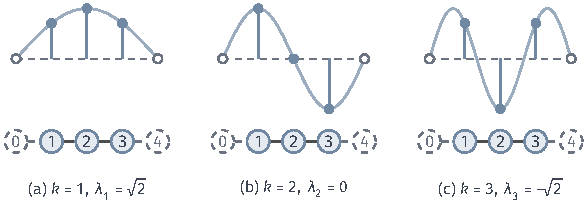
\includegraphics{figures/03-graphs/05-matrices-and-spectra/tikz/adjacency-path-sine-modes/figure.pdf}
  \caption{三点路径$P_3$上的三个正弦特征模式。底部虚线圆圈$0$和$4$为取零值的虚拟边界点，实线圆圈$1,2,3$为路径的实际顶点；上方曲线为$\sin(k\pi t/4)$，蓝色竖杆标出各顶点处的特征向量分量。(a) 基模$k=1$，$\lambda_1=\sqrt{2}$。(b) 二阶模$k=2$，$\lambda_2=0$。(c) 三阶模$k=3$，$\lambda_3=-\sqrt{2}$。}
  \label{fig:adjacency-path-sine-modes}
\end{BookInlineFigure}

\subsection{笛卡儿积图}
\label{sec:adjacency-cartesian-product-spectrum}

许多高维网格和超立方体图都可以由低维简单图通过笛卡儿积拼接而成。设$\mathcal G=(V_{\mathcal G},E_{\mathcal G})$和$\mathcal H=(V_{\mathcal H},E_{\mathcal H})$是两张图，它们的\term{笛卡儿积图}（Cartesian product of graphs）记为$\mathcal G\square\mathcal H$：其顶点集为笛卡儿积$V_{\mathcal G}\times V_{\mathcal H}=\{(u,v):u\in V_{\mathcal G},v\in V_{\mathcal H}\}$，两个顶点对$(u,v)$与$(u',v')$之间有边相连，当且仅当每次恰好沿着一个因子图走一步、另一个坐标保持不变：
\begin{itemize}
\item 要么第二坐标相同（$v=v'$），且第一坐标在$\mathcal G$中相邻（$\{u,u'\}\in E_{\mathcal G}$）；
\item 要么第一坐标相同（$u=u'$），且第二坐标在$\mathcal H$中相邻（$\{v,v'\}\in E_{\mathcal H}$）。
\end{itemize}

图~\ref{fig:adjacency-cartesian-edge-directions}展示了两个单边图$K_2$（顶点为$\{0,1\}$）的笛卡儿积$K_2\square K_2$：四个顶点对$(0,0),(1,0),(1,1),(0,1)$中，蓝色横边只改变第一坐标$u$，绿色竖边只改变第二坐标$v$，对角顶点$(0,0)$与$(1,1)$因同时改变了两个坐标而不相邻，最终围成四元环$C_4$。

\begin{BookInlineFigure}
  \centering
  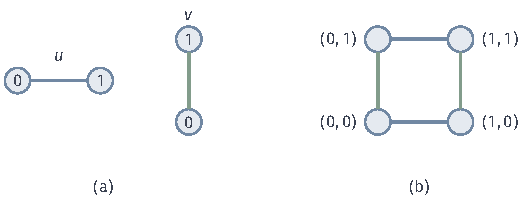
\includegraphics{figures/03-graphs/05-matrices-and-spectra/tikz/adjacency-cartesian-edge-directions/figure.pdf}
  \caption{两个单边图$K_2$的笛卡儿积$K_2\square K_2=C_4$。(a) 两个因子图分别提供第一坐标$u$与第二坐标$v$上的单步移动。(b) 蓝色横边只改变第一坐标$u$，绿色竖边只改变第二坐标$v$，四个顶点对围成四元环。}
  \label{fig:adjacency-cartesian-edge-directions}
\end{BookInlineFigure}

设$\mathcal G$有$p$个顶点、邻接矩阵为$\bm A_{\mathcal G}\in\mathbb R^{p\times p}$，$\mathcal H$有$q$个顶点、邻接矩阵为$\bm A_{\mathcal H}\in\mathbb R^{q\times q}$。按字典序排列$\mathcal G\square\mathcal H$的$pq$个顶点对：第一类边（改变$u$、保持$v$不变）对应的邻接作用是Kronecker积$\bm A_{\mathcal G}\otimes\bm I_q$；第二类边（保持$u$不变、改变$v$）对应的邻接作用是$\bm I_p\otimes\bm A_{\mathcal H}$。两类邻居相加，得到笛卡儿积图的邻接矩阵公式：
\begin{equation}
\bm A_{\mathcal G\square\mathcal H}
=\bm A_{\mathcal G}\otimes\bm I_q+\bm I_p\otimes\bm A_{\mathcal H}.
\label{eq:adjacency-cartesian-product}
\end{equation}

现在设$\bm x\in\mathbb R^p$是$\bm A_{\mathcal G}$属于特征值$\lambda$的特征向量（$\bm A_{\mathcal G}\bm x=\lambda\bm x$），$\bm y\in\mathbb R^q$是$\bm A_{\mathcal H}$属于特征值$\mu$的特征向量（$\bm A_{\mathcal H}\bm y=\mu\bm y$）。考察张量积向量$\bm x\otimes\bm y\in\mathbb R^{pq}$（它在顶点对$(u,v)$处的分量为乘积$x_u y_v$）。利用Kronecker积的混合乘积性质$(\bm M_1\otimes\bm M_2)(\bm x\otimes\bm y)=(\bm M_1\bm x)\otimes(\bm M_2\bm y)$，将$\bm A_{\mathcal G\square\mathcal H}$作用在$\bm x\otimes\bm y$上：
\[
\begin{aligned}
\bm A_{\mathcal G\square\mathcal H}(\bm x\otimes\bm y)
&=(\bm A_{\mathcal G}\bm x)\otimes(\bm I_q\bm y)+(\bm I_p\bm x)\otimes(\bm A_{\mathcal H}\bm y)\\
&=(\lambda\bm x)\otimes\bm y+\bm x\otimes(\mu\bm y)
=(\lambda+\mu)(\bm x\otimes\bm y).
\end{aligned}
\]
这表明$\bm x\otimes\bm y$是$\bm A_{\mathcal G\square\mathcal H}$的特征向量，对应的特征值恰好是两个因子特征值之和$\lambda+\mu$。分别取$\bm A_{\mathcal G}$的$p$个正交特征向量和$\bm A_{\mathcal H}$的$q$个正交特征向量，两两作Kronecker积共得到$pq$个两两正交的特征向量，张成整个$\mathbb R^{pq}$。

\begin{theorem}[笛卡儿积图的邻接谱]
\label{thm:adjacency-cartesian-product-spectrum}
设图$\mathcal G$的全部邻接特征值为$\lambda_1,\ldots,\lambda_p$（对应正交特征基$\bm x_1,\ldots,\bm x_p$），图$\mathcal H$的全部邻接特征值为$\mu_1,\ldots,\mu_q$（对应正交特征基$\bm y_1,\ldots,\bm y_q$）。则笛卡儿积图$\mathcal G\square\mathcal H$的全部$pq$个邻接特征值为两两之和
\[
\bigl\{\lambda_i+\mu_j:1\le i\le p,\;1\le j\le q\bigr\},
\]
其中$\lambda_i+\mu_j$对应的特征向量为$\bm x_i\otimes\bm y_j$。
\end{theorem}

定理~\ref{thm:adjacency-cartesian-product-spectrum}的一个经典应用是计算$d$维超立方体图$Q_d$的谱。$Q_d$的$2^d$个顶点是长度为$d$的$0$--$1$比特串$\{0,1\}^d$，两个比特串相邻当且仅当它们恰好在一个比特位上不同——这正是$d$个单边图$K_2$的连乘笛卡儿积$Q_d=K_2\square K_2\square\cdots\square K_2$。单边图$K_2$的两个特征值为$+1$和$-1$。在$d$个因子中各选一个特征值相加，若有$j$个因子选了$-1$、其余$d-j$个因子选了$+1$，则特征值之和为$(d-j)\cdot 1+j\cdot(-1)=d-2j$。从$d$个因子中挑出$j$个取$-1$共有$\binom{d}{j}$种选法，因此$Q_d$的特征值为$d-2j$（$j=0,1,\ldots,d$），重数为$\binom{d}{j}$。例如三维立方体$Q_3$的$8$个特征值为$3,1,1,1,-1,-1,-1,-3$。

\subsection{正则图的补图}
\label{sec:adjacency-complement-spectrum}

\begin{definition}[正则图]
\label{def:regular-graph}
若简单无向图$\mathcal G$的每个顶点都恰好有$d$个邻居（即所有顶点的度均等于$d$），则称$\mathcal G$为\term{$d$正则图}（$d$-regular graph）。
\end{definition}

在$d$正则图中，邻接矩阵$\bm A$的每一行都有$d$个$1$，行和恒等于$d$。因此给所有顶点统一赋读数$1$时，每个顶点的邻居读数之和都是$d$，即
\[
\bm A\bm 1=d\bm 1.
\]
这说明常向量$\bm 1$必定是$d$正则图属于特征值$d$的特征向量。又因$\bm A$是实对称矩阵，与常向量正交的零和子空间$\bm 1^\perp=\{\bm x\in\mathbb R^n:\bm 1^\top\bm x=0\}$在$\bm A$的作用下保持不变：对任意$\bm x\in\bm 1^\perp$，有$\bm 1^\top(\bm A\bm x)=(\bm A\bm 1)^\top\bm x=d(\bm 1^\top\bm x)=0$。于是我们可以在$\bm 1^\perp$内选出其余$n-1$个正交特征向量$\bm u_2,\ldots,\bm u_n$，这一性质使正则图的补图谱可以直接由原图谱换算出来。

\begin{theorem}[正则图的补图谱]
\label{thm:adjacency-regular-complement}
设$\mathcal G$是$n$个顶点的$d$正则简单无向图，其邻接特征值为$d=\lambda_1\ge\lambda_2\ge\cdots\ge\lambda_n$（其中$\lambda_1=d$对应常向量$\bm 1$，其余$\lambda_2,\ldots,\lambda_n$对应$\bm 1^\perp$中的正交特征向量$\bm u_2,\ldots,\bm u_n$）。则其补图$\overline{\mathcal G}$是$(n-1-d)$正则图，且$\overline{\mathcal G}$的全部邻接特征值为
\[
n-1-d\quad(\text{对应 }\bm 1),
\qquad\text{以及}\qquad
-1-\lambda_i\quad(i=2,\ldots,n,\text{ 对应 }\bm u_i).
\]
\end{theorem}

\begin{proof}
补图$\overline{\mathcal G}$保留相同的顶点集$V$，在所有互异且在原图$\mathcal G$中不相邻的顶点对之间连边。完全图的邻接矩阵为$\bm J-\bm I$，从中减去原图的邻接矩阵$\bm A_{\mathcal G}$，就得到补图的邻接矩阵：
\begin{equation}
\bm A_{\overline{\mathcal G}}=\bm J-\bm I-\bm A_{\mathcal G}.
\label{eq:adjacency-complement-matrix}
\end{equation}

分别考察$\bm A_{\overline{\mathcal G}}$在常向量$\bm 1$和在$\bm u_i\in\bm 1^\perp$（$i=2,\ldots,n$）上的作用：
\begin{itemize}
\item 在常向量$\bm 1$上，$\bm J\bm 1=n\bm 1$且$\bm A_{\mathcal G}\bm 1=d\bm 1$，故
\[
\bm A_{\overline{\mathcal G}}\bm 1=(\bm J-\bm I-\bm A_{\mathcal G})\bm 1=(n-1-d)\bm 1;
\]
\item 对每个$i\in\{2,\ldots,n\}$，因为$\bm u_i\in\bm 1^\perp$，有$\bm J\bm u_i=\bm 1(\bm 1^\top\bm u_i)=\bm 0$，且$\bm A_{\mathcal G}\bm u_i=\lambda_i\bm u_i$，故
\[
\bm A_{\overline{\mathcal G}}\bm u_i=(\bm J-\bm I-\bm A_{\mathcal G})\bm u_i=\bm 0-\bm u_i-\lambda_i\bm u_i=(-1-\lambda_i)\bm u_i.
\]
\end{itemize}
这$n$个正交特征向量给出了$\overline{\mathcal G}$的全部$n$个特征值。注意当原图$\mathcal G$不连通时，部分$i\geq 2$也可能满足$\lambda_i=d$，但由于$\bm u_i\in\bm 1^\perp$，它们在补图中均按$-1-\lambda_i=-1-d$换算。
\end{proof}

以四元环$C_4$（$n=4,d=2$）检验定理~\ref{thm:adjacency-regular-complement}：$C_4$的谱为$\lambda_1=2,\lambda_2=0,\lambda_3=0,\lambda_4=-2$。其补图$\overline{C_4}$只保留两条互不相交的对角边$\{1,3\}$与$\{2,4\}$（即$K_2\sqcup K_2$）。代入换算公式：常向量方向给出$n-1-d=4-1-2=1$；$\bm 1^\perp$中的三个特征值$0,0,-2$依次变为$-1-0=-1$、$-1-0=-1$、$-1-(-2)=1$。补图谱为$\{1,1,-1,-1\}$，与两条独立边各贡献一对$\pm1$完全一致。反之，若原图不是正则图，则$\bm A_{\mathcal G}\bm 1$的各分量是互不相等的顶点度，常向量$\bm 1$不再是$\bm A_{\mathcal G}$的特征向量，$\bm A_{\mathcal G}$与$\bm J$无法在常向量与$\bm 1^\perp$上同时对角化，上述简单换算公式便不再适用。
